\subsection{Semantic Code Search for Smart Contracts}
\label{subsec:semantic-code-search}

Penelitian yang dilakukan oleh \cite{shi2021semantic} mengusulkan model pencarian kode semantik untuk kontrak pintar yang disebut MM-SCS (Multi-Modal Smart Contract Code Search). Model ini dirancang untuk mengatasi masalah yang sering ditemui pada teknik pencarian kode tradisional, yaitu adanya jarak semantik antara kode dan query yang menghambat efektivitas pencarian. Penelitian ini fokus pada pengembangan model pencarian kode yang tidak hanya menggunakan representasi teks dari kode, tetapi juga memasukkan informasi alur kontrol dan data, yang sangat penting dalam konteks kontrak pintar yang kompleks.

\begin{figure}[ht]
  \centering
  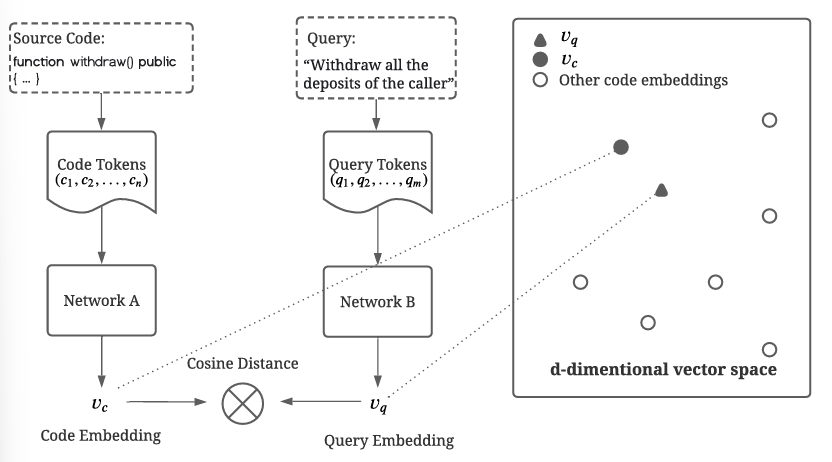
\includegraphics[width=0.7\textwidth]{resources/chapter-2/architecture-code-search.png}
  \caption{Arsitektur umum dari Neural Code Search \parencite{shi2021semantic}}
  \label{image:architecture-code-search}
\end{figure}

Dalam penelitian ini, MM-SCS mengintegrasikan Contract Elements Dependency Graph (CEDG) sebagai modalitas tambahan untuk menangkap informasi tentang alur data dan kontrol dalam kode. CEDG menggambarkan elemen-elemen utama dalam kode kontrak pintar, seperti variabel, fungsi, dan hubungan antar elemen tersebut, serta bagaimana elemen-elemen ini saling berinteraksi dalam kontrak pintar. Model ini juga mengadopsi teknik multi-head attention network untuk menghasilkan embedding dari fitur kode, yang memungkinkan model lebih fokus pada informasi konteks yang penting dalam kode.

Untuk memastikan efektivitas model meskipun data pelatihan terbatas, penulis menggunakan model ALBERT yang sudah dilatih sebelumnya dan disesuaikan untuk meningkatkan pemahaman konteks kode dalam pencarian semantik. Hasil eksperimen yang dilakukan menggunakan dataset yang berisi 470.000 pasangan kode dan deskripsi dari Github dan Etherscan menunjukkan bahwa MM-SCS mengungguli empat model state-of-the-art lainnya dalam hal Mean Reciprocal Rank (MRR) dan waktu pencarian, dengan peningkatan yang signifikan dalam akurasi pencarian kode pintar.

\begin{figure}[ht]
  \centering
  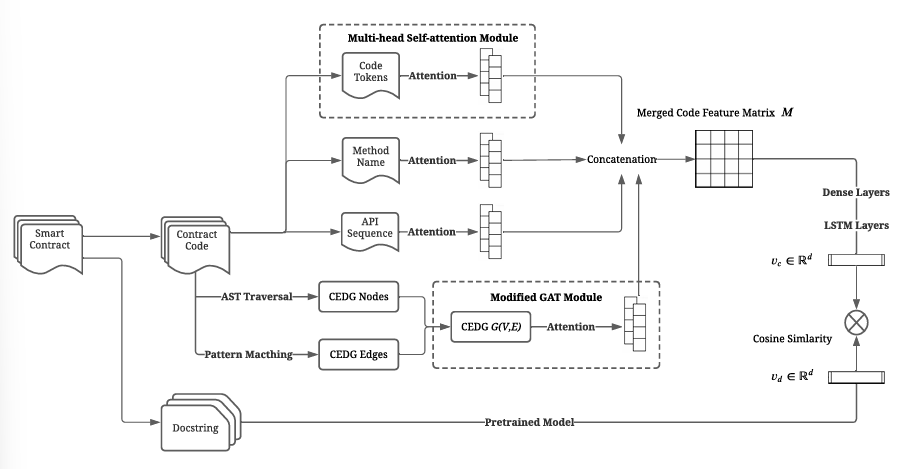
\includegraphics[width=0.7\textwidth]{resources/chapter-2/framework-mm-scs.png}
  \caption{Framework keseluruhan dari MM-SCS \parencite{shi2021semantic}}
  \label{image:framework-mm-scs}
\end{figure}

Penelitian ini memberikan kontribusi penting dalam meningkatkan pencarian kode semantik untuk kontrak pintar dengan memperkenalkan CEDG sebagai representasi grafis yang menggambarkan hubungan antar elemen kode dan menambahkan modalitas graf dalam pencarian semantik. Selain itu, eksperimen ini menunjukkan bahwa pendekatan MM-SCS memiliki keunggulan dibandingkan dengan model-model lainnya dalam hal akurasi dan efisiensi pencarian.

Hasil dari penelitian ini diharapkan dapat meningkatkan efisiensi pengembangan kontrak pintar dengan mempermudah pencarian dan penggunaan kembali potongan kode yang relevan dari repositori besar kode kontrak pintar.